\documentclass[parskip=full]{scrartcl}
\usepackage[top=2.5cm, bottom=2.5cm, left=2.5cm, right=2.5cm]{geometry}
\usepackage[utf8]{inputenc}
\usepackage[T1]{fontenc}
\usepackage[german]{babel}
\usepackage{hyperref}
\usepackage[toc, nonumberlist]{glossaries}
\usepackage{graphicx}
\usepackage{enumitem}
\usepackage{float}
\usepackage{color}

\title{OSIP - Softwaredesign}
\subtitle{OPC UA Simulator for Industrial Plants}
\author{
    M. Armbruster\\
    D. Kahles\\
    H. Lehmann\\
    M. Schwarzmann\\
    N. Wilhelm
}

\begin{document}
\maketitle

\vspace{20px}
\begin{center}
  
\includegraphics[scale=0.4]{../icon.png}
\end{center}
\pagebreak
\tableofcontents
\pagebreak

\section{Einleitung}
OSIP ist in drei große Pakete gegliedert: Simulation, Monitoring und Core.
Simulation realisiert die Fertigungssimulation und Monitoring die Überwachungskonsole.
Core beinhaltet gemeinsame Unterpakete vom Fertigungssimulation und Monitoring sowie Unterpakete zu IO und der Implementierung
von OPC UA.
Das grundlegende Entwurfsmuster Model-View-Controller (MVC) ist bis auf das Model zweifach für die Fertigungssimulation und die Überwachungskonsole verwirklicht, die getrennt von einander existieren.
Das gemeinsame Model befindet sich in Core. Dabei benutzt die Überwachungskonsole nur core.base und core.behavior.
Die Fertigungssimulation benutzt ein erweitertes Model aus den Unterpakteten core.simulation, core.base und core.behavior.
Das Unterpaket core.simulation ist für das Mischen von Farben und die Simulation der Verbindungsrohre zuständig.

\section{Klassenbeschreibungen}
Die Klassenbeschreibungen können im Anhang dieses Dokuments gefunden werden.

\section{Abläufe}
\subsection{Wrapper für OPC UA}

\subsubsection{Server-Wrapper}
\begin{figure}[H]
  \centering
  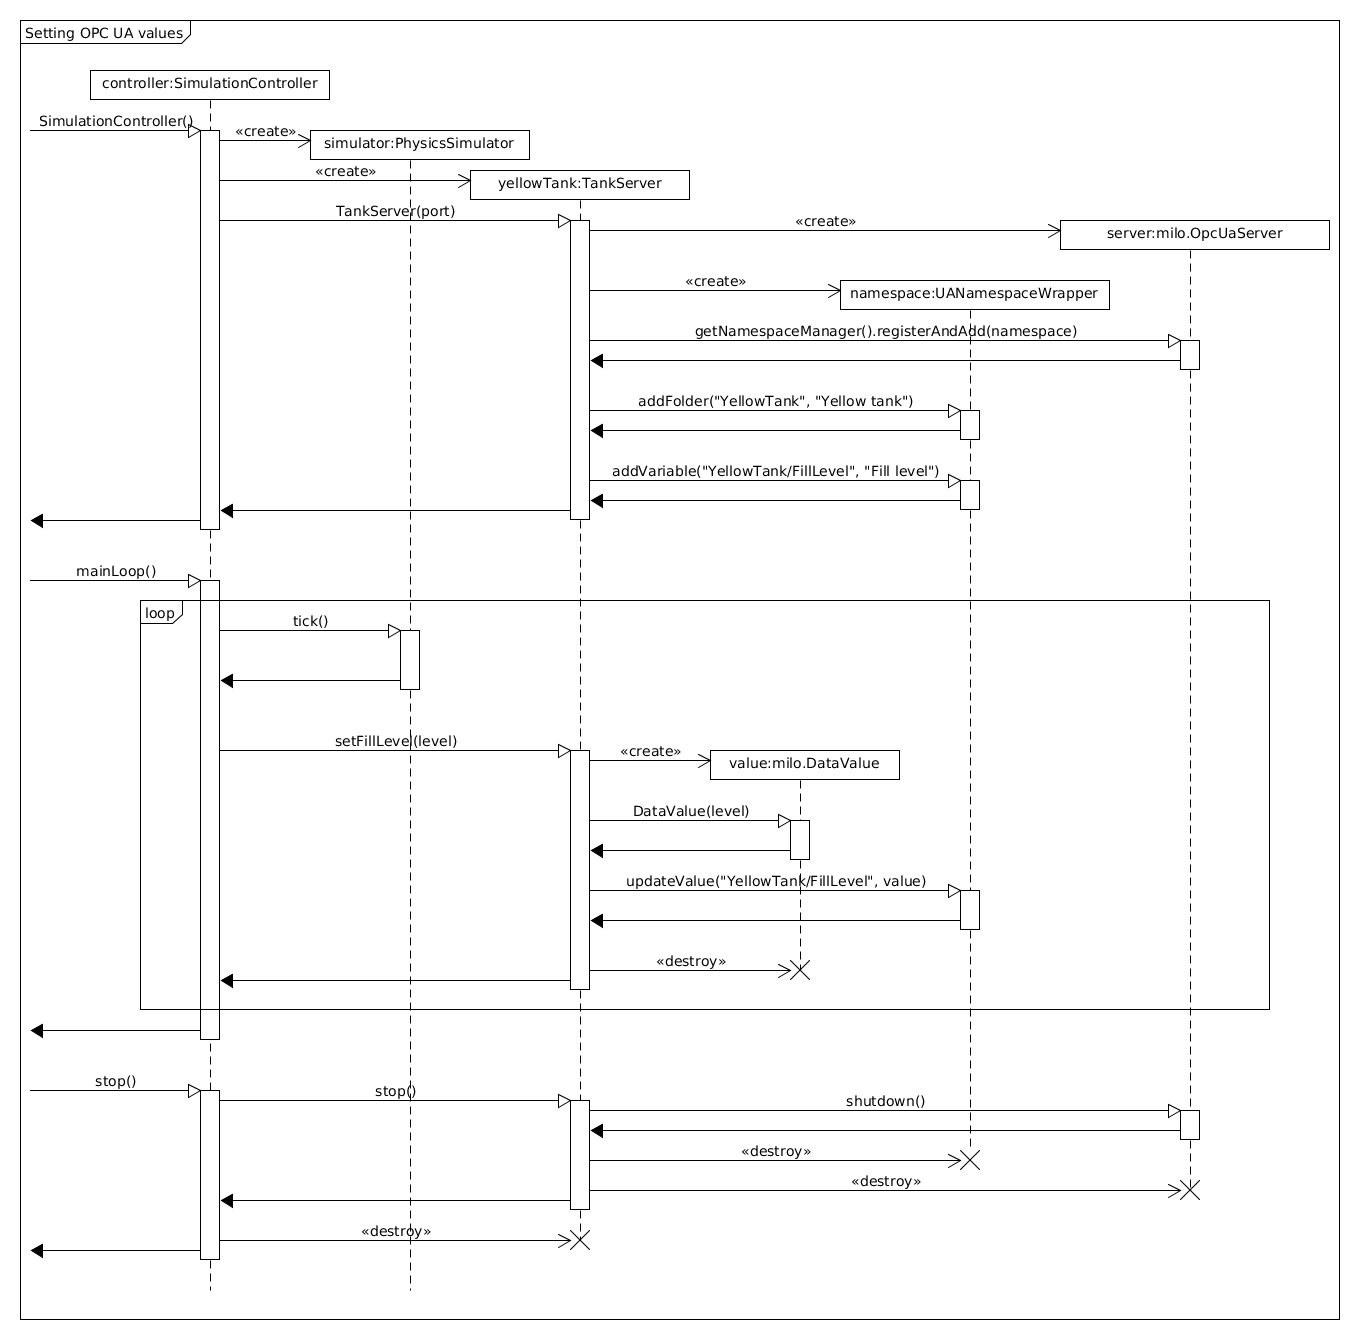
\includegraphics[scale=0.35]{design/sequence-diagrams/sequence-set-server-value.png}
  \caption{Setzen von Werten über den server wrapper}
\end{figure}

\subsubsection{Client-Wrapper}
\begin{figure}[H]
  \centering
  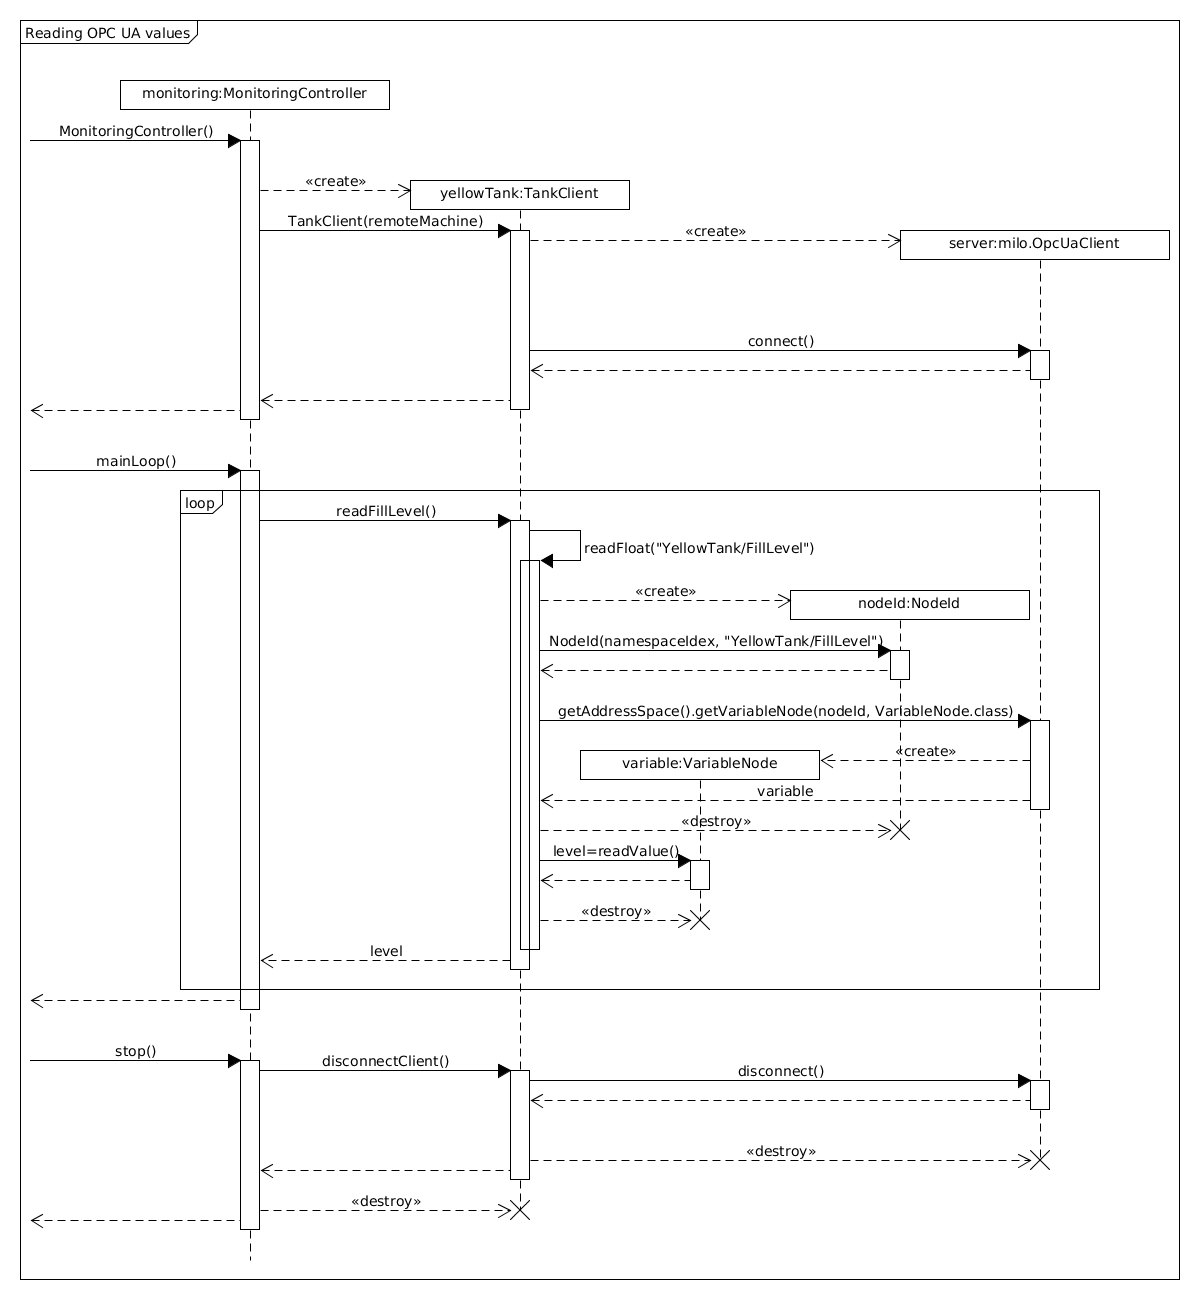
\includegraphics[scale=0.34]{design/sequence-diagrams/sequence-read-client-value.png}
  \caption{Lesen von Werten über den client wrapper}
\end{figure}

\subsection{Neuzeichnen der GUI der Simulation}
\begin{figure}[H]
  \centering
  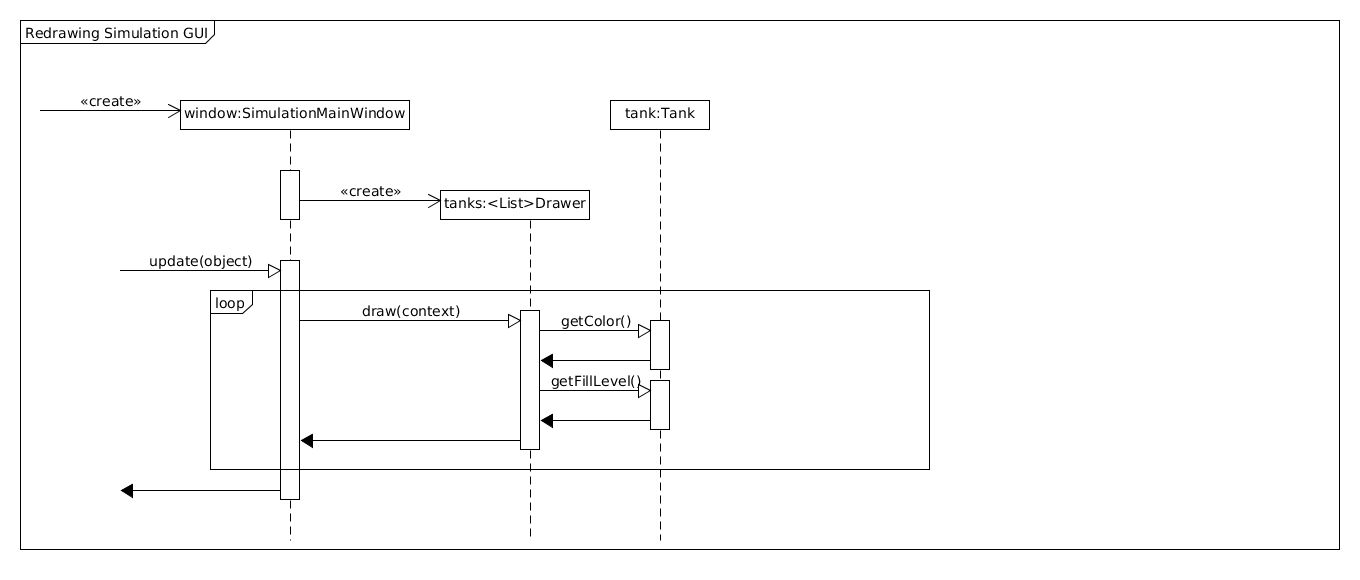
\includegraphics[scale=0.35]{design/sequence-diagrams/simulation-redraw.png}
  \caption{Neuzeichnen der GUI der Simulation}
\end{figure}

\subsection{Berechnen der Tank-Simulation}
\begin{figure}[H]
  \centering
  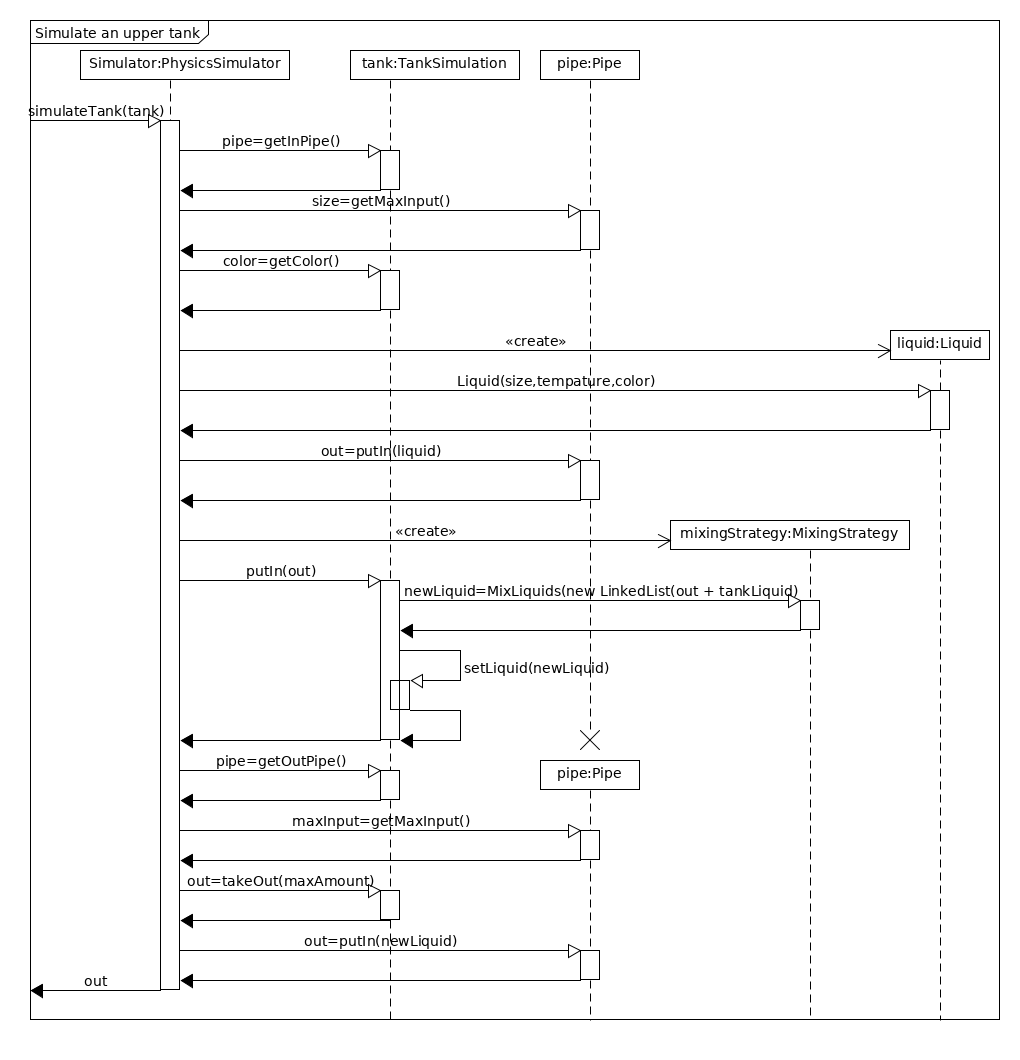
\includegraphics[scale=0.45]{design/sequence-diagrams/tank-simulation.png}
  \caption{Berechnen der Tank-Simulation}
\end{figure}

\subsection{Einstellungen aus der Datei erhalten und verwenden}
\begin{figure}[H]
  \centering
  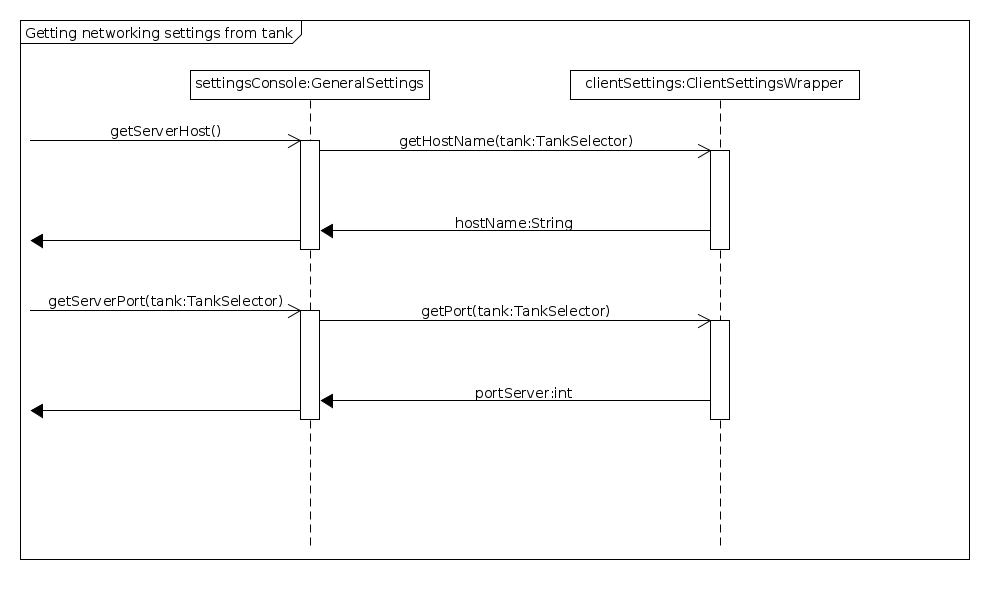
\includegraphics[scale=0.4]{design/sequence-diagrams/getting-networking-settings.png}
  \caption{Einstellungen aus der Datei erhalten und verwenden}
\end{figure}


\section{Änderungen zum Pflichtenheft}

\subsection{\"Ubernommene Kann-Kriterien}
Im folgenden werden die Kann-Kriterien aus dem Pflichtenheft noch einmal alle aufgelistet. Zu jedem der Kriterien wird
kurz zusammengefasst, was genau es bedeutet. Es werden erst die implementierten und anschlie{\ss}end die nicht implementierten
Kriterien gelistet.

\subsubsection{Implementierte Kann-Kriterien}
Die implementierten Kann-Kriterien sind wie folgt:

\begin{itemize}
    \item Sowohl in der \"Uberwachungskonsole als auch in der Fertigungssimulation werden Fehler bei der Programmausf\"uhrung
    nach stdout geloggt. Die Logs werden nicht persistiert.
    \item In der Fertigungssimulation k\"onnen vorgefertigte Simulationsszenarien geladen werden. Diese sind in eigenen Dateien definiert.
    Die Ausführung der Simulationsszenarien f\"uhrt dazu, dass die Steuervariablen sich nach Vorgaben des Szenarios ohne
    weitere Aktion des Benutzers \"andern.
    \item In den Zuflusswerten der Fertigungssimulation ist ein Jitter eingebaut. Dieser sorgt f\"ur leichte Variationen in den
    Zuflussmengen und der Temperatur der Zufl\"usse. Das Ausma{\ss} des Jitters ist nicht einstellbar.
    \item Innerhalb der \"Uberwachungskonsole kann der Benutzer selbst einstellen, in welchem Zeitintervall die Werte der
    Fertigungssimulation abgefragt werden. Alle Werte werden im jeweils gleichen Intervall abgefragt.
    \item Die Alarme in der \"Uberwachungskonsole k\"onnen vom Benutzer jeweils einzeln zu- und abgeschaltet werden. Die Menge der
    aktivierten Alarme wird bei Beenden der \"Uberwachungskonsole persistiert. Beim n\"achsten Start der \"Uberwachungskonsole
    werden die gleichen Alarme automatisch wieder aktiviert.
    \item Die Alarme, die von der \"Uberwachungskonsole empfangen werden, werden in einer Textausgabe innerhalb der
    \"Uberwachungskonsole geloggt.
\end{itemize}

\subsubsection{Nicht implementierte Kann-Kriterien}
Die nicht implementierten Kann-Kriterien sind wie folgt:

\begin{itemize}
    \item Es stehen keine verschiedenen Sprachoptionen f\"ur \"Uberwachungskonsole und Fertigungssimulation zur Verf\"ugung.
    Die einzige vorhandene Sprache ist Englisch. Durch die Verwendung von i18n ist die Anwendung allerdings leicht übersetzbar.
    \item Die vorgegebenen Alarme k\"onnen nicht ver\"andert werden. Insbesondere ist es nicht m\"oglich, eigene Alarme hinzuzuf\"ugen
    oder die Schwellenwerte der vorgegebenen Alarme zu modifizieren.
    \item Der Jitter in den Simulationswerten ist fest vorgegeben und kann in seiner Intensit\"at nicht ver\"andert werden.
    \item Fehler bei der Programmausf\"uhrung werden nicht in eine Datei geschrieben.
\end{itemize}

\section{Klassendiagramme}
Die Klassendiagramme können im Anhang dieses Dokuments gefunden werden.

\section{Verwendete Entwurfsmuster}
% Aufzählen: Geheimnisprinzip, MVC etc.

\end{document}
